\documentclass[a4paper, 12pt]{article} % 12pt, A4 page

% packages
\usepackage{amsmath,amssymb} % math symbols
\usepackage{amsfonts} % 〃    〃
\usepackage{amsthm} % math proofs
\usepackage{xcolor} % text coloring
\usepackage{setspace} % spacing
\usepackage{graphicx} % image
\usepackage{cite} % BibTex
\usepackage[notlof,nottoc,numbib]{tocbibind} % somehow makes the references appear in ToC

\newcommand{\researchquestion}{How can vector calculus be used to model and analyze incompressible fluid flow in two-dimensional spaces, and what insights can this provide about the vector fields of real-world fluid systems with circular obstacles?}
\graphicspath{ {resources/} }

% custom commands
\newcommand{\ihat}{\hat{\imath}} % i hat
\newcommand{\jhat}{\hat{\jmath}} % j hat
\newcommand{\fatf}{\mathbf{F}} % for Vector field F
\newcommand{\justify}[1]{\text{\color{gray}(#1)}}
\newcommand{\definedas}{\stackrel{\Delta}{=}} % definitions
\newcommand{\referto}[1]{\textsuperscript{\color{darkgray}\tiny[see \ref{#1}]}} % definitions
% > derivatives
\newcommand{\der}[2]{\frac{\mathrm{d} #1}{\mathrm{d} #2}} % derivative
\newcommand{\partialder}[2]{\frac{\partial #1}{\partial #2}} % partial derivative
\newcommand{\materialder}[2]{\frac{\mathrm{D} #1}{\mathrm{D} #2}} % material derivative
% > vector calculus operators
\DeclareMathOperator{\gradient}{\nabla} % gradient operator
\DeclareMathOperator{\divergence}{\nabla\cdot} % divergence operator
\DeclareMathOperator{\curl}{\nabla\times} % divergence operator

\renewcommand{\qedsymbol}{\hfill\ensuremath{\blacksquare}}

% formatting
\doublespacing % double spacing
\pagenumbering{arabic} % page numbering

% theorems
\newtheorem{greenstheorem}{Green's theorem}

\begin{document}
\begin{titlepage} % title page
	\begin{center}
		\vspace*{0.5cm}
		\Large
		\textbf{\researchquestion}

		\vspace{1.5cm}
		\large
		\textbf{Mathematics AA HL}

		\vfill{}\color{darkgray}
		Word Count: 556 % (maximum 4000)
	\end{center}
\end{titlepage}

\tableofcontents\newpage % table of contents

% INTRODUCTION
\section{Introduction}
Vector calculus provides the foundation and tools for the analysis and modeling of several real-world phenomona, and is integral to understanding several important fields such as aero- \& hydrodynamics, as well as the modeling of weather \& climates. 

Through the use of pure mathematics, this essay will investigate the flow of fluids in 2 dimensional spaces around circular obstacles. Visual representations through mediums such as vector field plots (plotted through a custom program
% > aim & scope
\subsection{Aim \& scope}
This essay will for simplicity's sake only cover fluid flow around circular obstacles in $\mathbb{R}^2$ spaces; an alaysis of fluid flow in $\mathbb{R}^3$ spaces would be much more complex.
Furthermore, only incompressible fluids sans sinks and sources ($\fatf\ni\divergence\fatf=0$), will be analyzed.

Most of the analysis will take place using Green's theorem\referto{sec:greenstheorem}.

% > background
\subsection{Background}
\subsubsection{Partial derivatives}
One dimensional calculus provides the tools for finding the slope of some function $f$ with respect to some variable $x$ at some point through the derivative, often denoted by Leibniz's notation $\der{f}{x}$, representing the ratio between some small change in $f$ after some small change in $x$. For example, the equation of the slope of the function $f(x)=x^2$ at some point can be calculated using the formal definition of a deriative:
\begin{equation}
	\der{f}{x}=\underbrace{\lim_{h\rightarrow0}\frac{f(x+h)-f(x)}{h}}_\text{\hidewidth The formal definition of a derivative\hidewidth}\\
\end{equation}
\begin{align*}
	f(x)=x^2\rightarrow\der{f}{x}&=\lim_{h\rightarrow0}\frac{(x+h)^2-(x)^2}{h}\\
	&=\lim_{h\rightarrow0}\frac{x^2+2xh+h^2-x^2}{h}\\
	&=\lim_{h\rightarrow0}\frac{2xh+h^2}{h}\\
	&=\lim_{h\rightarrow0}2x+h=2x
\end{align*}
More conveniently, Lagrange's or Euler's notation for the derivative is often used to avoid excessive writing.
$$\der{f}{x}\equiv f'(x)\equiv \mathrm{D}f$$
For the purposes of this essay, the formal definition of a derivative will not be used to calculate each derivation, rather common patterns and rules (such as the power rule, product rule, etc.) will be used. 

Multi-variable calculus introduces the partial derivative, which functions the same as a normal derivative but treats all variables except for the one being differentiated by as constants, allowing for the derivation of multi-variable functions.
\begin{align*}
	f(x,y)=x^2+y^2\implies\partialder{f}{x}=2x && \justify{power rule}
\end{align*}
However, the partial derivative only provides part of the picture, since it only takes into consideration one variable. Defining one single full picture "derivative" of a multi-variable function is not possible, since there are an infinite number of "slopes" at some point, and what you want the derivative to achieve will depend on your goal (e.g. what direction you want to differentiate in).

\subsubsection{The nabla operator}
The nabla operator, denoted $\nabla$ (pronounced nabla or del), is a vector filled with partial derivatives with respect to each variable some function $f$ takes. For example, consider some function $f:\mathbb{R}^n\rightarrow\mathbb{R}^m$, nabla would then be defined as:
\begin{equation}
	\left.\nabla=
	\begin{bmatrix}
		\partialder{}{x} \\
		\partialder{}{y} \\
		\partialder{}{z} \\ 
		\vdots 	         \\
	\end{bmatrix}
	\color{gray}\right\} \color{gray}n\text{ times}\color{black}
\end{equation}
Nabla gives the vector pointing in the direction of greatest ascent\referto{p:nablagreatestchange}. For example, aplying this to our previous example $f(x,y)=x^2+y^2$ results in:
$$\nabla f=\begin{bmatrix}
	\partialder{}{x}x^2+y^2\\
	\partialder{}{y}x^2+y^2	
\end{bmatrix}=\begin{bmatrix}
	2x\\
	2y
\end{bmatrix}$$
Meaning that at some point $(x,y)$, the direction of steepest incline will be:$$2{\begin{bmatrix}x\\y\end{bmatrix}}$$
The gradient of a function is often visualized as a vector field, plotting the vector field of the previous example yields:

\begin{figure}[!ht]
	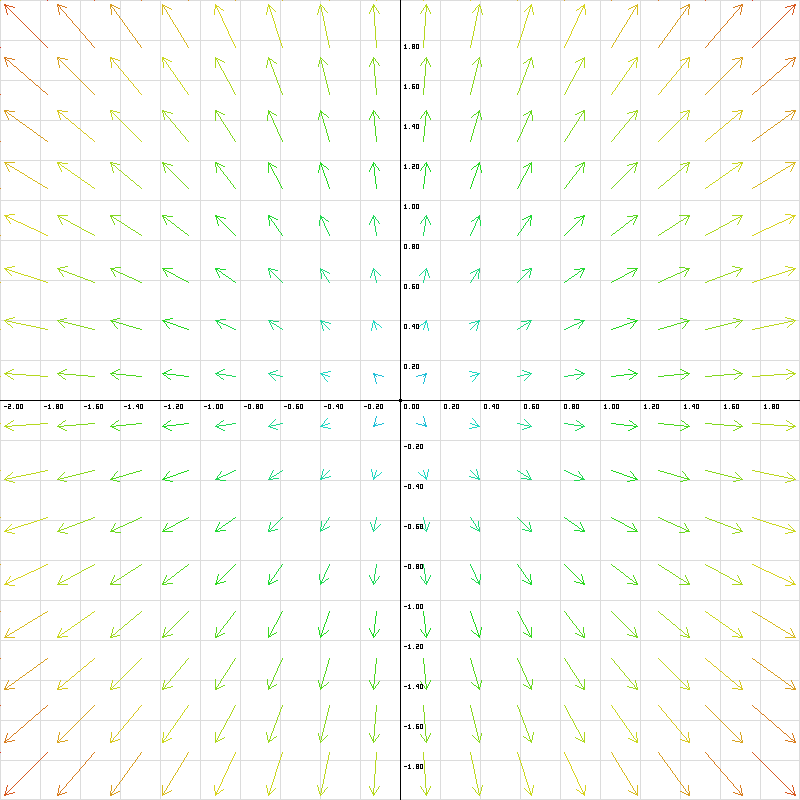
\includegraphics[scale=0.45]{x2y2.png}
	\centering
	\caption{Vector field for $f(x,y)=\begin{bmatrix}2x\\2y\end{bmatrix}$}
	\label{fig:x2y2}
\end{figure}

The nabla operator proves foundational to several important concepts within vector calculus, as will be demonstrated.

\subsubsection{Directional derivatives}
Partial derivatives allow for the computation of derivatives in the $x$ and $y$, and this concept may be extended to the derivative in any direction $\vec{v}$. Since $\nabla f$ computes the rate of change in the $x$ and $y$ directions, dotting this vector with some directional vector $\vec{v}$ gives the directional derivative in the direction of $\vec{v}$, denoted as:
\begin{equation}
	\nabla_{\vec{v}}f=\nabla f\cdot\vec{v}
\end{equation}
Nabla pointing in the direction of greatest ascent can be proven using the directional derivative.
\begin{proof}\label{p:nablagreatestchange}
	\begin{align*}
		\nabla_{\vec{v}}f&=\nabla f\cdot\vec{v}\\
		\max\nabla_{\vec{v}}f&\rightarrow\text{direction of greatest change}\\
		\max\nabla_{\vec{v}}f&=\max\nabla f\cdot\vec{v}\\
		&=\max\lVert\nabla f\rVert\lVert\vec{v}\rVert\cos{\theta}\\
		&\leadsto\theta=0\\
		&\implies\max\nabla_{\vec{v}}f\text{ points in the direction of }\nabla f
	\end{align*}
\end{proof}
\subsubsection{Other}
$$f:\mathbb{R}^n\rightarrow\mathbb{R}^n\ni n>1,n\in\mathbb{Z}$$
\begin{equation}
	\materialder{f}{t}\definedas\partialder{f}{t}+\underbrace{\vec{v}\cdot\nabla f}_{\hidewidth\text{Directional derivative }\nabla_{\vec{v}}f\hidewidth}
\end{equation}
$$\vec{v_1}\otimes\vec{v_2}$$

% > fluid dynamics
\subsection{Fluid dynamics}
An incompressible fluid is any fluid such that $\divergence\fatf=0$, which is to say that the divergence of the fluid is 0.

% > the navier-stokes equations
\subsection{Green's theorem}\label{sec:greenstheorem}
\begin{greenstheorem}
	The double integral over some reigon $R$ of the curl of a vector field $\fatf$ is equal to the line integral over some curve $C$ of $\fatf$
	$$\int_C \mathbf{F} \cdot d\mathbf{r} = \iint_R \left( \frac{\partial Q}{\partial x} - \frac{\partial P}{\partial y} \right) \, dA$$
	$$\iint_R\curl\fatf\mathrm{d}A=\oint_C\fatf\cdot\mathrm{d}\mathbf{r}$$
\end{greenstheorem}
\begin{equation} % navier-stokes
	\materialder{f}{\mathbf{t}}=\iiint\limits_{V}(\materialder{\rho}{\mathbf{t}}+\rho(\nabla\cdot u))dV
\end{equation}
Lorem ipsum dolor sit amet \cite{peyret2012computational}

% references
\newpage
\bibliographystyle{apalike}
\bibliography{sources}
\stepcounter{section}
\addcontentsline{toc}{section}{\protect\numberline{\thesection}List of Figures}
\renewcommand{\listfigurename}{\thesection\hspace{20pt}List of Figures}\listoffigures

% testing
\newpage
$$\fatf(t):\mathbb{R}\rightarrow\mathbb{R}^2$$
$$\leadsto\mathbf{P}(t, \vec{p})=\vec{p}+\hat{\imath}\iint_0^t\fatf_x\ \mathrm{d}t+\hat{\jmath}\iint_0^t\fatf_y\ \mathrm{d}t$$
$$\mathbf{P}(t, \vec{p})=\vec{p}+\iint_0^t\hat{\imath}\fatf_x+\hat{\jmath}\fatf_y\ \mathrm{d}t$$
$$\jhat+\ihat$$
\begin{align*}
	A&=B\\
	 &=C && \text{substitution}
\end{align*}
\begin{proof} Green's Theorem
	\begin{align*}
		B \definedas C \span \\
		A&=B \\
		 &=C \\
	\end{align*}
\end{proof}
$$a\underbrace{a}_\text{banana}$$
\end{document}